\section{Metodologia}

A metodologia deste trabalho consiste em seis etapas que podem ser vistas na
Figura \ref{fig:metodologia}.

\graphicspath{{figuras/}}

\begin{figure}[!h]
 \centering
 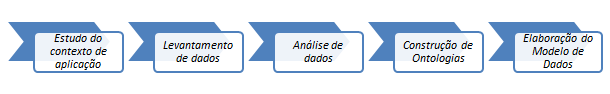
\includegraphics[scale = 0.75]{metodologia}
 \caption{Etapas do trabalho}
 \label{fig:metodologia}

\end{figure}
\textit{Estudo do contexto de aplicação}: essa etapa consiste na análise do contexto, dos
usuários e do ambiente WEB ao qual a proposta será aplicada.

\textit{Levantamento de dados}: essa etapa consiste na revisão de literatura e busca por
ontologias e terminologias já existentes relacionadas a acidentes e aos dados das
ocorrências no World Wide Web Consortium (W3C). O levantamento das ontologias
ocorrerá por meio de duas expressões de busca, em sites de busca e em bases de dados, na
língua inglesa, para obtenção de um resultado mais abrangente.

\begin{center}
  Expressão 1: “Car accident ontology”\\
  Expressão 2: “Traffic accident ontology”
\end{center}


\textit{Análise de dados}: essa etapa consiste na leitura dos artigos e verificação das
ontologias encontradas para garantir que estejam alinhadas aos objetivos.

\textit{Estruturação da Ontologia}: essa etapa consiste na elaboração de um modelo conceitual
referente a ontologia.

\textit{Construção de Ontologias}: essa etapa consiste na construção de uma ontologia de
acidentes para o contexto do trabalho, baseada em ontologias existentes e na estruturação realizada.

\textit{Planejamento da aplicação da Ontologia no Software}: essa etapa consiste na elaboração de um Planejamento
de como a ontologia completa será finalizada e integrada ao ``Pé na Estrada''

